\subsection{Comparison of Prediction Methods}

EG01-EG23, EG01-EG24, EG01-EG29, and EG01-EG30 transition scenarios
are set up in \Cyclus using \deploy. 
To determine the most effective \deploy prediction methods for 
each transition scenario, a
comparison of the use of each prediction method in each 
transition scenarios is conducted. 

Similar to the basic transition scenarios, these transition scenario 
simulations begin with an initial fleet of \gls{LWR}s and after 
80 years, the simulation progressively decommissions the \gls{LWR}s. 
\deploy is set up to have a constant power demand of 60GW and to 
deploy \gls{PWR}s that use \gls{MOX} fuel and \gls{SFR} reactors 
depending on the transition scenario. 

Figure \ref{fig:eg2324} and Figure \ref{fig:eg2930} 
show the set up of facilities and mass flows for 
each transition scenario in \Cyclus. 

\begin{figure}[]
	\centering
	\begin{subfigure}[t]{\textwidth}
		\centering
		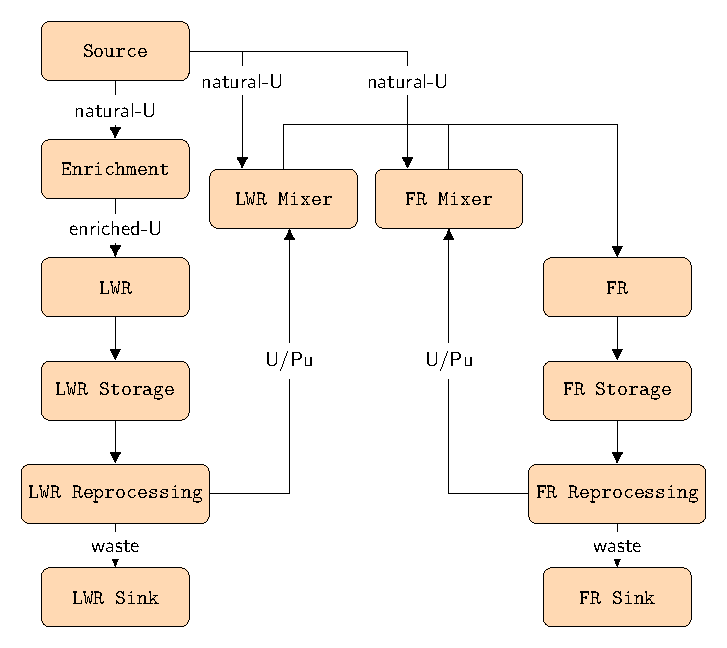
\includegraphics[width=0.55\linewidth]{23flow.pdf} 
		\caption{EG01-EG23.}
		\label{fig:23flow}
	\end{subfigure}
	\vspace{1cm}
	\begin{subfigure}[t]{\textwidth}
		\centering
		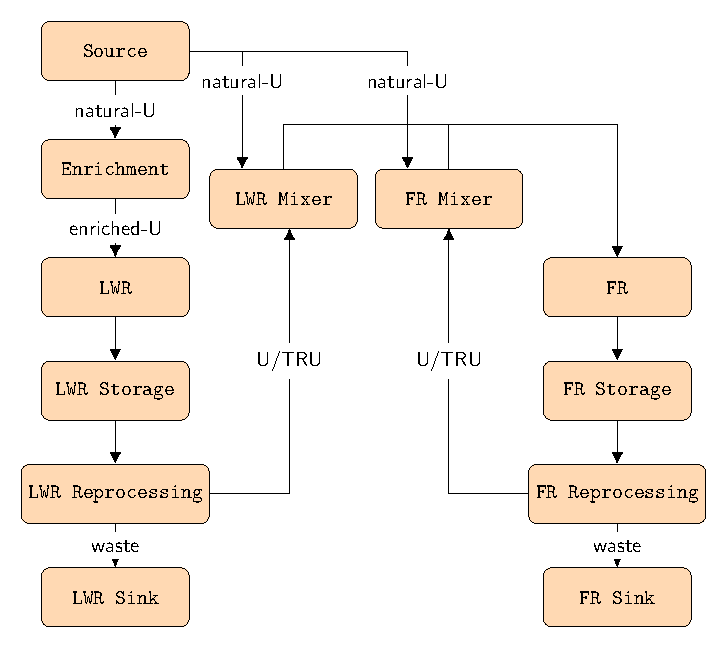
\includegraphics[width=0.55\linewidth]{24flow.pdf} 
		\caption{EG01-EG24.}
		\label{fig:24flow}
	\end{subfigure}
	\hfill
	\caption{Diagrams with facilities and mass flow of the scenarios EG01-EG23 and EG01-EG24.}
	\label{fig:eg2324}
\end{figure}

\begin{figure}[]
	\centering
	\begin{subfigure}[t]{\textwidth}
		\centering
		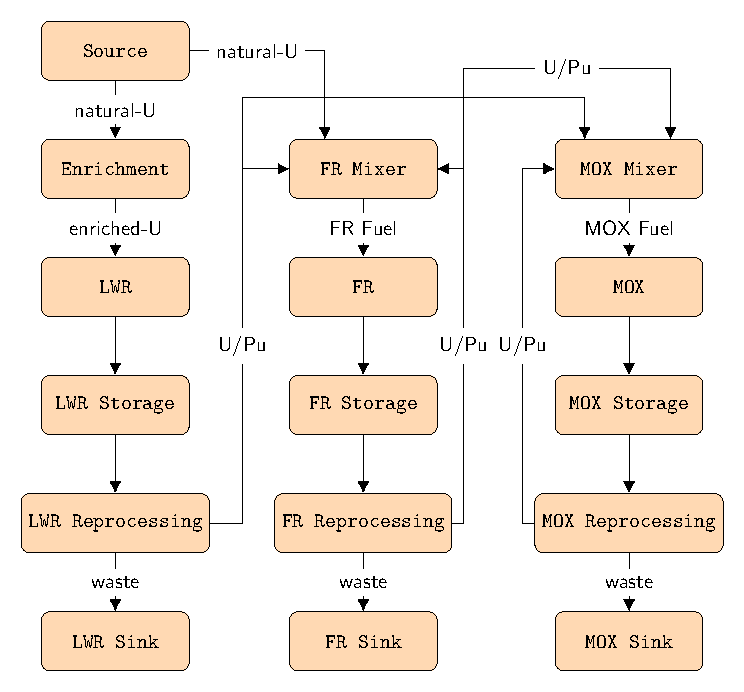
\includegraphics[width=0.55\linewidth]{29flow.pdf} 
		\caption{EG01-EG29.}
		\label{fig:29flow}
	\end{subfigure}
	\vspace{1cm}
	\begin{subfigure}[t]{\textwidth}
		\centering
		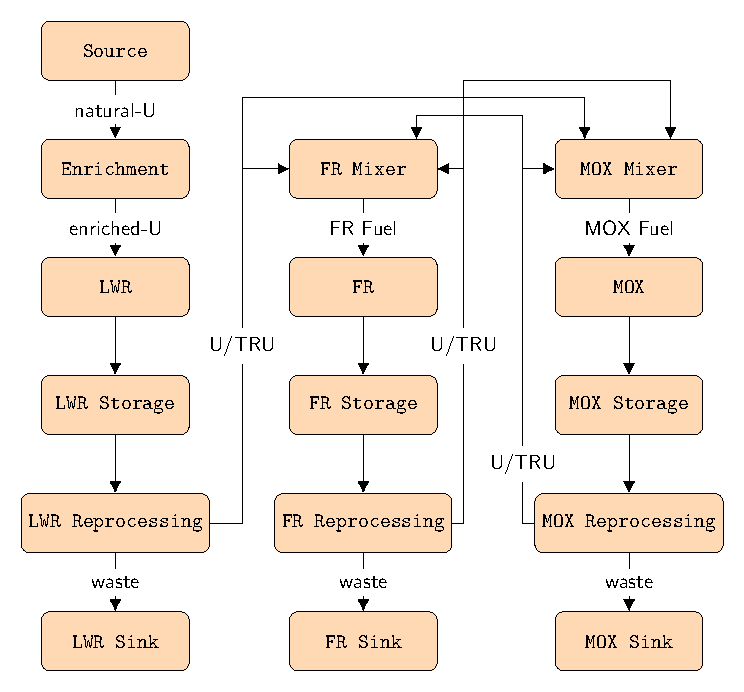
\includegraphics[width=0.55\linewidth]{30flow.pdf} 
		\caption{EG01-EG30.}
		\label{fig:30flow}
	\end{subfigure}
	\hfill
	\caption{Diagrams with facilities and mass flow of the scenarios EG01-EG29 and EG01-EG30.}
	\label{fig:eg2930}
\end{figure}

Table xx shows the number of time steps with power undersupply, 
cumulative undersupply and oversupply magnitudes for power for 
EG01-EG23 transition scenario. 
The ideal transition scenario eliminates power undersupply and 
minimizes power oversupply. 

\begin{table}[]
	\centering
	\caption {Undersupply and oversupply of Power for the different algorithms used to calculate EG01-EG23.}
	\label{tab:23-power}
	\begin{tabular}{|l|c|c|c|}
		\hline
		& \multicolumn{3}{c|}{Power} \\ \hline
		Algorithm & \shortstack{No. of time steps\\of undersupply}  & 
		\shortstack{Cumulative\\Undersupply[GW]}  & \shortstack{Cumulative\\Oversupply[GW]} \\ \hline
		MA        & 20 	& 20.0  &  920.5   \\ \hline
		ARMA      & 18 	&  7.7  &  1036.5  \\ \hline
		ARCH      &  0 	&   0  	&  1320.1  \\ \hline
		POLY      &  1 	&  0.3 	&  1783.5  \\ \hline
		EXP\_SMOOTHING 	& 20 	& 11.0 & 1473.5 \\ \hline
		HOLT-WINTERS  	& 20 	& 11.0 & 1473.5 \\ \hline
		FFT       & 2 	& 60.3 	& 1751.9 	\\ \hline
		SW\_SEASONAL    & 20 	& 18.6 	& 1119.9 	\\ \hline
	\end{tabular}
\end{table}

\subsection{Sensitivity Analysis}

\subsection{Best Performance Models}
Table %\ref{tab:bestinputs} 
shows \deploy input parameters for
EG01-EG23, EG01-EG24, EG01-EG29, and EG01-EG30 transition scenarios
that ensure there is no undersupply of power and minimizes 
the undersupply and under capacity of the other facilities. 
The need for buffers for commodities is a reflection of reality
in which ideally a supply cushion exists to ensure that there 
is available supply in the case of unexpected undersupply. 

%INSERT TABLE \ref{tab:bestinputs}%
Table \ref{tab:bestundersupply} shows the

%INSERT TABLE \ref{tab:undersupply}%